% questions.tex —— 2015 年·重庆卷·理工农医类 · 题目内容片段（无答案）
% 由 tools/generate_projects.py 依来源总账自 2015/2015_数学真题_重庆理_试题.md 生成，勿手改（改源 MD 后重跑）


\begin{gktip}
来源说明：固定源为 2 页 A3 扫描件，印刷页 939–940，卷内无答案。卷首无注意事项框、无「第Ⅰ卷」字样；第 1 题题干末无答题括号，第 5 题题干「体积」后缺「为」，第 13 题「A 的角平分线」前无角符号，第 17 题「外观完全相同」与「从中任意选取」间无标点，均照录不补。

图形说明：第 3、5、7、14、19、21 题图依原页拓扑重绘，不按比例。
\end{gktip}

\begin{gktip}
卷面抬头：2015 普通高等学校招生考试（重庆卷理）

（源疑点：扫描件卷首只有上述标题行，其后直接为「一、选择题」；无注意事项说明框，也无「第Ⅰ卷」「第Ⅱ卷」字样。两页页脚印刷页码分别为 939、940。此处照扫描页记录，未按常见卷式补写。）

（源疑点：第 5 题题干在扫描页上止于「则该几何体的体积」，其后直接为三视图与选项，未见「为」字；此处照录，未补字。）

（源疑点：第 13 题「$A$ 的角平分线」在扫描页上未见「$\angle$」符号；此处照录，未补符号。）

（源疑点：第 17 题「外观完全相同」与「从中任意选取」之间扫描页未见标点；此处照录，未补标点。）
\end{gktip}

\gkpart{一、选择题}

\begin{question}
\gkti{1}已知集合 $A=\{1,2,3\}$，$B=\{2,3\}$，则

（A）$A=B$；（B）$A\cap B=\varnothing$；（C）$A\subsetneqq B$；（D）$B\subsetneqq A$。

\end{question}
\begin{question}
\gkti{2}在等差数列 $\{a_{n}\}$ 中，若 $a_{2}=4$，$a_{4}=2$，则 $a_{6}=$（　）。

（A）$-1$；（B）$0$；（C）$1$；（D）$6$。

\Needspace{0.4\textheight}
\end{question}
\begin{question}
\gkti{3}重庆市 $2013$ 年各月的平均气温（$^\circ$C）数据的茎叶图如下：
\nopagebreak[4]
\begin{center}% 2015 年重庆卷（理工农医类）第 3 题：平均气温数据的茎叶图（依固定扫描页重绘，只画拓扑与标号，不按比例）
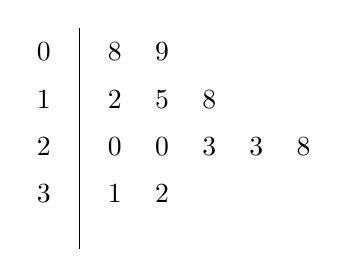
\begin{tikzpicture}[scale=1.0]
  % 茎叶分隔线
  \draw (0,2.55)--(0,-0.25);
  % 茎 0
  \node at (-0.45,2.25) {$0$};
  \node at (0.45,2.25) {$8$};
  \node at (1.05,2.25) {$9$};
  % 茎 1
  \node at (-0.45,1.65) {$1$};
  \node at (0.45,1.65) {$2$};
  \node at (1.05,1.65) {$5$};
  \node at (1.65,1.65) {$8$};
  % 茎 2
  \node at (-0.45,1.05) {$2$};
  \node at (0.45,1.05) {$0$};
  \node at (1.05,1.05) {$0$};
  \node at (1.65,1.05) {$3$};
  \node at (2.25,1.05) {$3$};
  \node at (2.85,1.05) {$8$};
  % 茎 3
  \node at (-0.45,0.45) {$3$};
  \node at (0.45,0.45) {$1$};
  \node at (1.05,0.45) {$2$};
\end{tikzpicture}
\end{center}
\nopagebreak[4]
则这组数据的中位数是（　）。

（A）$19$；（B）$20$；（C）$21.5$；（D）$23$。

\end{question}
\begin{question}
\gkti{4}“$x>1$”是“$\log_{\frac{1}{2}}(x+2)<0$”的（　）。

（A）充要条件；（B）充分不必要条件；（C）必要而不充分条件；（D）既不充分也不必要条件。

\Needspace{0.4\textheight}
\end{question}
\begin{question}
\gkti{5}某几何体的三视图如图所示，则该几何体的体积（　）。
\nopagebreak[4]
\begin{center}% 2015 年重庆卷（理工农医类）第 5 题：某几何体的三视图（依固定扫描页重绘，只画拓扑与标号，不按比例）
\begin{tikzpicture}[>=stealth,scale=1.0]
  % 正视图：右侧 2×1 矩形，左侧接直角三角形（水平边 1、竖直边 1）
  \draw (0,0) rectangle (2,1);
  \draw (-1,0)--(0,1);
  \draw (-1,0)--(0,0);
  % 正视图尺寸标注
  \draw[<->] (-1,-0.4)--(0,-0.4);
  \node at (-0.5,-0.75) {$1$};
  \draw[<->] (0,-0.4)--(2,-0.4);
  \node at (1,-0.75) {$2$};
  \draw[<->] (2.28,0)--(2.28,1);
  \node at (2.62,0.5) {$1$};
  \node at (0.5,-1.25) {正视图};
  % 左视图：半径 1 的半圆，竖直半径与两条弦
  \draw (4.1,0)--(6.1,0);
  \draw (4.1,0) arc (180:0:1);
  \draw (5.1,0)--(5.1,1);
  \draw (5.1,1)--(4.1,0);
  \draw (5.1,1)--(6.1,0);
  \node at (5.1,-1.0) {左视图};
  % 俯视图：2×2 矩形，左侧接等腰三角形（底 2、高 1）
  \draw (0,-4) rectangle (2,-2);
  \draw (-1,-3)--(0,-2)--(0,-4);
  \draw (-1,-3)--(0,-3);
  % 俯视图尺寸标注（深度方向 1+1）
  \draw[<->] (0.3,-2)--(0.3,-3);
  \node at (0.62,-2.5) {$1$};
  \draw[<->] (0.3,-3)--(0.3,-4);
  \node at (0.62,-3.5) {$1$};
  \draw[<->] (0,-4.35)--(2,-4.35);
  \node at (1,-4.75) {$2$};
  \node at (0.5,-5.35) {俯视图};
\end{tikzpicture}
\end{center}
\nopagebreak[4]
（A）$\dfrac{1}{3}+\pi$；（B）$\dfrac{2}{3}+\pi$；（C）$\dfrac{1}{3}+2\pi$；（D）$\dfrac{2}{3}+2\pi$。

\end{question}
\begin{question}
\gkti{6}若非零向量 $\boldsymbol{a}$，$\boldsymbol{b}$ 满足 $|\boldsymbol{a}|=\dfrac{2\sqrt{2}}{3}|\boldsymbol{b}|$，且 $(\boldsymbol{a}-\boldsymbol{b})\perp(3\boldsymbol{a}+2\boldsymbol{b})$，则 $\boldsymbol{a}$ 与 $\boldsymbol{b}$ 的夹角为（　）。

（A）$\dfrac{\pi}{4}$；（B）$\dfrac{\pi}{2}$；（C）$\dfrac{3\pi}{4}$；（D）$\pi$。

\Needspace{0.4\textheight}
\end{question}
\begin{question}
\gkti{7}执行如图所示的程序框图，若输出 $k$ 的值为 $8$，则判断框内可填入的条件是（　）。
\nopagebreak[4]
\begin{center}% 2015 年重庆卷（理工农医类）第 7 题：程序框图（依固定扫描页重绘，只画拓扑与标号，不按比例）
\begin{tikzpicture}[>=stealth,scale=0.85]
  % 开始
  \draw[rounded corners=6pt] (-1.0,11.6) rectangle (1.0,12.4);
  \node at (0,12.0) {开始};
  \draw[->] (0,11.6)--(0,11.2);
  % 赋初值
  \draw (-1.8,10.4) rectangle (1.8,11.2);
  \node at (0,10.8) {$s=0,\ k=0$};
  \draw[->] (0,10.4)--(0,8.1);
  % 判断框（空白）
  \draw (-1.9,7.4)--(0,6.7)--(1.9,7.4)--(0,8.1)--cycle;
  % 否
  \draw[->] (0,6.7)--(0,6.0);
  \node at (0.35,6.35) {否};
  \draw (-1.4,6.0)--(1.4,6.0)--(1.2,5.2)--(-1.6,5.2)--cycle;
  \node at (-0.1,5.6) {输出 $k$};
  \draw[->] (0,5.2)--(0,4.6);
  \draw[rounded corners=6pt] (-1.0,4.6) rectangle (1.0,3.8);
  \node at (0,4.2) {结束};
  % 是：先 k=k+2，再 s=s+1/k，回到判断框上方
  \draw[->] (1.9,7.4)--(4.6,7.4)--(4.6,7.9);
  \node at (2.4,7.78) {是};
  \draw (3.5,7.9) rectangle (5.7,8.7);
  \node at (4.6,8.3) {$k=k+2$};
  \draw[->] (4.6,8.7)--(4.6,9.1);
  \draw (3.4,9.1) rectangle (5.8,9.9);
  \node at (4.6,9.5) {$s=s+\frac{1}{k}$};
  \draw[->] (4.6,9.9)--(4.6,10.2)--(0,10.2);
\end{tikzpicture}
\end{center}
\nopagebreak[4]
（A）$s\le\dfrac{3}{4}$；（B）$s\le\dfrac{5}{6}$；（C）$s\le\dfrac{11}{12}$；（D）$s\le\dfrac{25}{24}$。

\end{question}
\begin{question}
\gkti{8}已知直线 $l$：$x+ay-1=0$（$a\in\mathbf{R}$）是圆 $C$：$x^{2}+y^{2}-4x-2y+1=0$ 的对称轴．过点 $A(-4,a)$ 作圆 $C$ 的一条切线，切点为 $B$，则 $|AB|=$（　）。

（A）$2$；（B）$4\sqrt{2}$；（C）$6$；（D）$2\sqrt{10}$。

\end{question}
\begin{question}
\gkti{9}若 $\tan\alpha=2\tan\dfrac{\pi}{5}$，则 $\dfrac{\cos\left(\alpha-\dfrac{3\pi}{10}\right)}{\sin\left(\alpha-\dfrac{\pi}{5}\right)}=$（　）。

（A）$1$；（B）$2$；（C）$3$；（D）$4$。

\end{question}
\begin{question}
\gkti{10}设双曲线 $\dfrac{x^{2}}{a^{2}}-\dfrac{y^{2}}{b^{2}}=1$（$a>0$，$b>0$）的右焦点为 $F$，右顶点为 $A$，过 $F$ 作 $AF$ 的垂线与双曲线交于 $B$，$C$ 两点，过 $B$，$C$ 分别作 $AC$，$AB$ 的垂线，两垂线交于点 $D$．若 $D$ 到直线 $BC$ 的距离小于 $a+\sqrt{a^{2}+b^{2}}$，则该双曲线的渐近线斜率的取值范围是（　）。

（A）$(-1,0)\cup(0,1)$；（B）$(-\infty,-1)\cup(1,+\infty)$；（C）$(-\sqrt{2},0)\cup(0,\sqrt{2})$；（D）$(-\infty,-\sqrt{2})\cup(\sqrt{2},+\infty)$。

\end{question}
\gkpart{二、填空题}

\begin{question}
\gkti{11}设复数 $a+bi$（$a,b\in\mathbf{R}$）的模为 $\sqrt{3}$，则 $(a+bi)(a-bi)=$\gkblank{}。

\end{question}
\begin{question}
\gkti{12}$\left(x^{3}+\dfrac{1}{2\sqrt{x}}\right)^{5}$ 的展开式中 $x^{8}$ 的系数是\gkblank{}。（用数字作答）

\end{question}
\begin{question}
\gkti{13}在 $\triangle ABC$ 中，$B=120^\circ$，$AB=\sqrt{2}$，$A$ 的角平分线 $AD=\sqrt{3}$，则 $AC=$\gkblank{}。

\Needspace{0.4\textheight}
\end{question}
\begin{question}
\gkti{14}如图，圆 $O$ 的弦 $AB$，$CD$ 相交于点 $E$，过点 $A$ 作圆 $O$ 的切线与 $DC$ 的延长线交于点 $P$，若 $PA=6$，$AE=9$，$PC=3$，$CE:ED=2:1$，则 $BE=$\gkblank{}。
\nopagebreak[4]
\begin{center}% 2015 年重庆卷（理工农医类）第 14 题：圆 O 的两条相交弦与过 A 的切线（依固定扫描页重绘，只画拓扑与标号，不按比例）
% 按题设 PA=6、PC=3、CE:ED=2:1、AE=9 数值定形：CD 为不过圆心的弦，E 在 CD 上，O 在 CD 上方
\begin{tikzpicture}[>=stealth,scale=0.55]
  \coordinate (P) at (-9,0);
  \coordinate (C) at (-6,0);
  \coordinate (E) at (0,0);
  \coordinate (D) at (3,0);
  \coordinate (O) at (-1.5,3.7125);
  \coordinate (A) at (-7,5.6569);
  \coordinate (B) at (1.5556,-1.2571);
  % 圆 O
  \draw (O) circle (5.8338);
  % 切线 PA
  \draw (P)--(A);
  % 割线 P-C-E-D
  \draw (P)--(D);
  % 弦 AB
  \draw (A)--(B);
  % 标号
  \fill (P) circle (1.2pt) node[below left] {$P$};
  \fill (C) circle (1.2pt) node[below left] {$C$};
  \fill (D) circle (1.2pt) node[above right] {$D$};
  \fill (E) circle (1.2pt) node[below] {$E$};
  \fill (B) circle (1.2pt) node[below right] {$B$};
  \fill (O) circle (1.2pt) node[right] {$O$};
  \fill (A) circle (1.2pt) node[fill=white,inner sep=1pt,above left=1pt] {$A$};
\end{tikzpicture}
\end{center}
\nopagebreak[4]
\end{question}
\begin{question}
\gkti{15}已知直线 $l$ 的参数方程为

\nopagebreak[4]
\[
\begin{cases}
x=-1+t,\\
y=1+t
\end{cases}
\quad (t\ \text{为参数}),
\]

以坐标原点为极点，$x$ 轴的正半轴为极轴建立极坐标系，曲线 $C$ 的极坐标方程为 $\rho^{2}\cos 2\theta=4$（$\rho>0$，$\dfrac{3\pi}{4}<\theta<\dfrac{5\pi}{4}$），则直线 $l$ 与曲线 $C$ 的交点的极坐标为\gkblank{}。

\end{question}
\begin{question}
\gkti{16}若函数 $f(x)=|x+1|+2|x-a|$ 的最小值为 $5$，则实数 $a=$\gkblank{}。

\end{question}
\gkpart{三、解答题}

\begin{question}
\gkti{17}端午节吃粽子是我国的传统习俗．设一盘中装有 $10$ 个粽子，其中豆沙粽 $2$ 个，肉粽 $3$ 个，白粽 $5$ 个，这三种粽子的外观完全相同从中任意选取 $3$ 个．

（1） 求三种粽子各取到 $1$ 个的概率；

（2） 设 $X$ 表示取到的豆沙粽个数，求 $X$ 的分布列与数学期望．

\end{question}
\begin{question}
\gkti{18}已知函数 $f(x)=\sin\left(\dfrac{\pi}{2}-x\right)\sin x-\sqrt{3}\cos^{2}x$．

（1） 求 $f(x)$ 的最小正周期和最大值；

（2） 讨论 $f(x)$ 在 $\left[\dfrac{\pi}{6},\dfrac{2\pi}{3}\right]$ 上的单调性．

\Needspace{0.4\textheight}
\end{question}
\begin{question}
\gkti{19}如图，三棱锥 $P-ABC$ 中，$PC\perp$ 平面 $ABC$，$PC=3$，$\angle ACB=\dfrac{\pi}{2}$，$D$，$E$ 分别为线段 $AB$，$BC$ 上的点，且 $CD=DE=\sqrt{2}$，$CE=2EB=2$．

（1） 证明：$DE\perp$ 平面 $PCD$；

（2） 求二面角 $A-PD-C$ 的余弦值．
\nopagebreak[4]
\begin{center}% 2015 年重庆卷（理工农医类）第 19 题：三棱锥 P-ABC，D 在 AB 上，E 在 BC 上（依固定扫描页重绘，只画拓扑与标号，不按比例）
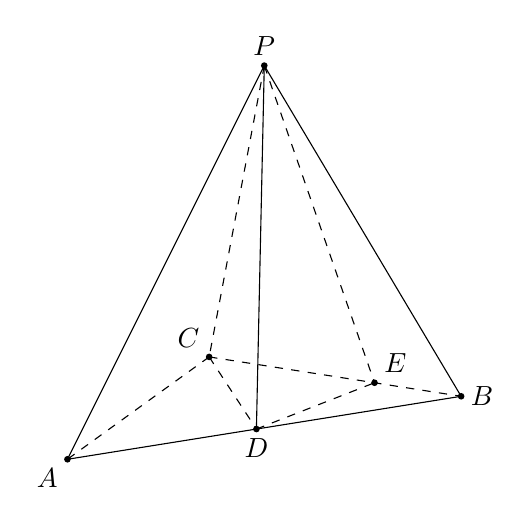
\begin{tikzpicture}[>=stealth,scale=1.0]
  % 顶点与底面各点
  \coordinate (P) at (4.0,6.0);
  \coordinate (A) at (1.5,1.0);
  \coordinate (C) at (3.3,2.3);
  \coordinate (B) at (6.5,1.8);
  \coordinate (D) at (3.9,1.384);
  \coordinate (E) at (5.4,1.972);
  % 实线棱
  \draw (P)--(A);
  \draw (P)--(B);
  \draw (P)--(D);
  \draw (A)--(B);
  % 虚线：PC、PE、CA、CB、CD、DE
  \draw[dashed] (P)--(C);
  \draw[dashed] (P)--(E);
  \draw[dashed] (C)--(A);
  \draw[dashed] (C)--(B);
  \draw[dashed] (C)--(D);
  \draw[dashed] (D)--(E);
  % 标号
  \fill (P) circle (1.2pt) node[above] {$P$};
  \fill (A) circle (1.2pt) node[below left] {$A$};
  \fill (B) circle (1.2pt) node[right] {$B$};
  \fill (C) circle (1.2pt) node[above left] {$C$};
  \fill (D) circle (1.2pt) node[below] {$D$};
  \fill (E) circle (1.2pt) node[above right] {$E$};
\end{tikzpicture}
\end{center}
\nopagebreak[4]
\end{question}
\begin{question}
\gkti{20}设函数 $f(x)=\dfrac{3x^{2}+ax}{\mathrm{e}^{x}}$（$a\in\mathbf{R}$）．

（1） 若 $f(x)$ 在 $x=0$ 处取得极值，确定 $a$ 的值，并求此时曲线 $y=f(x)$ 在点 $(1,f(1))$ 处的切线方程；

（2） 若 $f(x)$ 在 $[3,+\infty)$ 上为减函数，求 $a$ 的取值范围．

\Needspace{0.4\textheight}
\end{question}
\begin{question}
\gkti{21}如图，椭圆 $\dfrac{x^{2}}{a^{2}}+\dfrac{y^{2}}{b^{2}}=1$（$a>b>0$）的左、右焦点分别为 $F_{1}$，$F_{2}$，过 $F_{2}$ 的直线交椭圆于 $P$，$Q$ 两点，且 $PQ\perp PF_{1}$．

（1） 若 $|PF_{1}|=2+\sqrt{2}$，$|PF_{2}|=2-\sqrt{2}$，求椭圆标准方程；

（2） 若 $|PF_{1}|=|PQ|$，求椭圆的离心率 $e$．
\nopagebreak[4]
\begin{center}% 2015 年重庆卷（理工农医类）第 21 题：椭圆与过右焦点的弦 PQ（依固定扫描页重绘，只画拓扑与标号，不按比例）
\begin{tikzpicture}[>=stealth,scale=1.0]
  % 坐标轴
  \draw[->] (-3.9,0)--(4.1,0) node[below] {$x$};
  \draw[->] (0,-2.3)--(0,2.7) node[left] {$y$};
  \node[below left] at (0,0) {$O$};
  % 椭圆
  \draw[domain=0:360,samples=120] plot ({3*cos(\x)},{1.8*sin(\x)});
  % 焦点与点
  \coordinate (F1) at (-2,0);
  \coordinate (F2) at (2,0);
  \coordinate (P) at (1.268,1.631);
  \coordinate (Q) at (2.462,-1.028);
  % 弦 PQ 与线段 PF1
  \draw (P)--(Q);
  \draw (P)--(F1);
  % 直角标记（PF1 与 PQ 在 P 处）
  \draw (1.071,1.533)--(1.161,1.332)--(1.358,1.430);
  % 标号
  \fill (F1) circle (1.2pt) node[below] {$F_{1}$};
  \fill (F2) circle (1.2pt) node[below left] {$F_{2}$};
  \fill (P) circle (1.2pt) node[above left] {$P$};
  \fill (Q) circle (1.2pt) node[right] {$Q$};
\end{tikzpicture}
\end{center}
\nopagebreak[4]
\end{question}
\begin{question}
\gkti{22}在数列 $\{a_{n}\}$ 中，$a_{1}=3$，$a_{n+1}a_{n}+\lambda a_{n+1}+\mu a_{n}^{2}=0$（$n\in\mathbf{N}_{+}$）．

（1） 若 $\lambda=0$，$\mu=-2$，求数列 $\{a_{n}\}$ 的通项公式；

（2） 若 $\lambda=\dfrac{1}{k_{0}}$（$k_{0}\in\mathbf{N}_{+}$，$k_{0}\ge 2$），$\mu=-1$，证明：$2+\dfrac{1}{3k_{0}+1}<a_{k_{0}+1}<2+\dfrac{1}{2k_{0}+1}$．

\end{question}